\documentclass[7pt]{article}
\usepackage[left=1in, right=1in, top=1in, bottom=1in]{geometry}
\usepackage[latin1]{inputenc}
\usepackage{amsmath}
\usepackage{amsfonts}
\usepackage{amssymb}
\usepackage{graphicx}
\usepackage{caption} 
\author{Ben Larson}
\title{Homework 6 }
\date{Oct 20, 2016} 
\begin{document}
	\maketitle
	\section{Nelder-Mead Method}
	Nelder-Mead is a derivative free algorithm that works by minimizing a function based on a simplex model. f(x) is found for 3 arbitrary points, then based on the results the algorithm will experiment on a point estimated from the best, worst, and second best value of the simplex. We discard the worst point and re-run the algorithm. The transformations that the simplex can have is a reflection, expansion and contraction. These transformations use the geometry, ordering, and centroid to calculate/estimate new values. These are derivative free, but still have a similar process as gradient based optimization. \\
	For this problem we solved the function:
	$$ f(x) = x_1^2+x_2^2+x_1x_2+x_1x_3+x_3x^2 $$
	I implemented the Nelder-Mead algorithm as found in the website using matlab: 
%	$http://www.scholarpedia.org/article/Nelder-Mead_algorithm
	The results were as follows: 
	\noindent%
	\begin{minipage}{\linewidth}% to keep image and caption on one page
		\makebox[\linewidth]{%        to center the image
			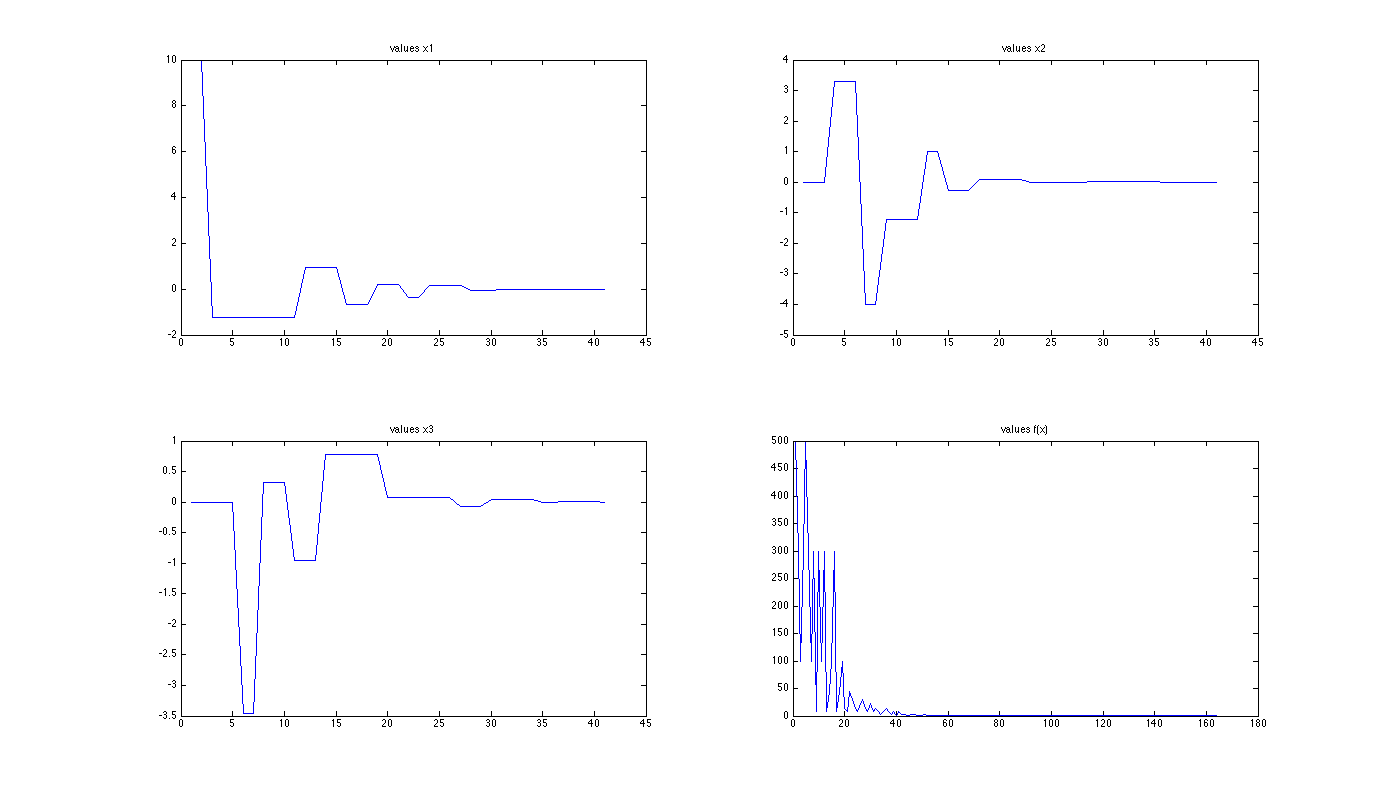
\includegraphics[keepaspectratio=true,scale=0.5]{nelder.png}}
		\captionof{figure}{We can see that the x1,x2,x3 all come closer to zero as the algorithm progresses. At zero they kinda bounce around until the termination conditions are met. The bottom right plot is the function evaluated at the newly minimized (x1,x2,x3). Notice it approaches zero as the algorithm progresses.}\label{visina8}%      only if needed  
	\end{minipage}

	
	\section{Nelder-Mead, quasi-Newton, and conjugate gradient}
	For this section we compare the implemented algorithms. For the Bleale function I show a contour and the march of the algorithm towards the minimum. However, with the higher dimensions of the Rosenbrock function I only show the values evaluated at the function f(x). 
		\subsection{Beale's Function}
		Of all the algorithms Conjugate gradient minimizes in the fewest steps. \\
			\noindent%
			\begin{minipage}{\linewidth}% to keep image and caption on one page
				\makebox[\linewidth]{%        to center the image
					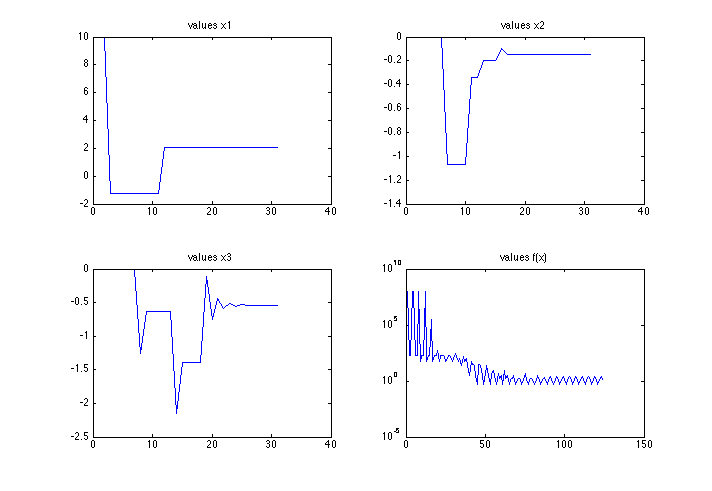
\includegraphics[keepaspectratio=true,scale=0.5]{nelder_bleal.png}}
				\captionof{figure}{Nelder-Mead optimizing the Bleale function.}   
			\end{minipage}
		\noindent%
		\begin{minipage}{\linewidth}% to keep image and caption on one page
			\makebox[\linewidth]{%        to center the image
				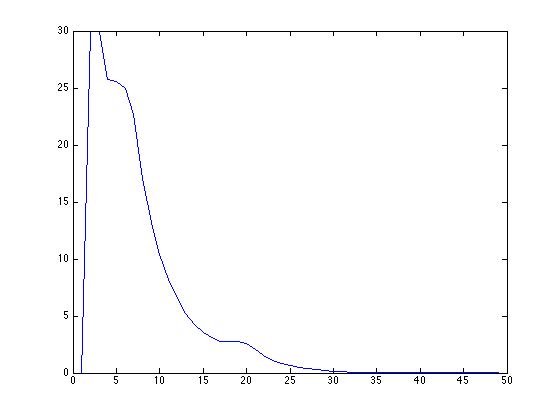
\includegraphics[keepaspectratio=true,scale=0.5]{bfgs_bleal.png}}
			\captionof{figure}{Quasi-Newton BFGS optimizing the Bleale function.}   
		\end{minipage}
		\noindent%
		\begin{minipage}{\linewidth}% to keep image and caption on one page
			\makebox[\linewidth]{%        to center the image
				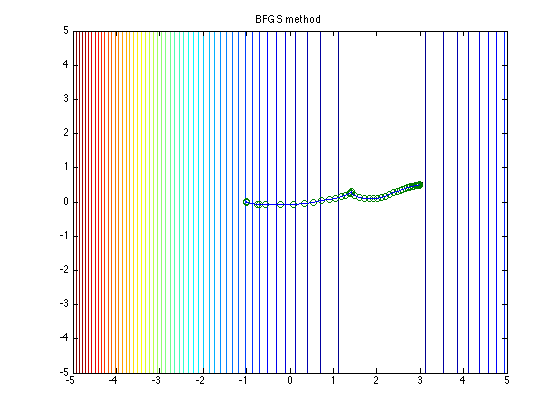
\includegraphics[keepaspectratio=true,scale=0.5]{2dbleal-bfgs.png}}
			\captionof{figure}{Contour plot of the BFGS method on the Bleale optimization.}   
		\end{minipage}
			\noindent%
			\begin{minipage}{\linewidth}% to keep image and caption on one page
				\makebox[\linewidth]{%        to center the image
					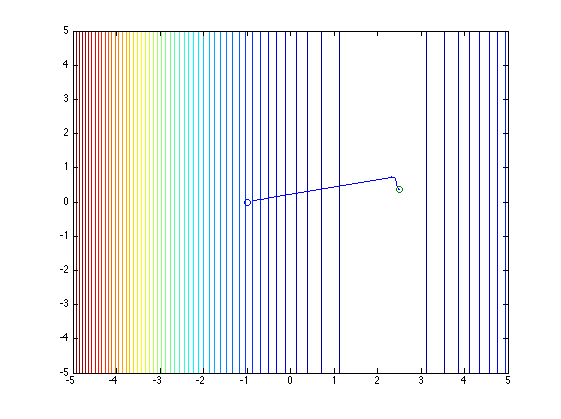
\includegraphics[keepaspectratio=true,scale=0.5]{conjGrad_bleal.png}}
				\captionof{figure}{Conjugate Gradient optimizing the Bleale function.}   
			\end{minipage}
			\noindent%
			\begin{minipage}{\linewidth}% to keep image and caption on one page
				\makebox[\linewidth]{%        to center the image
					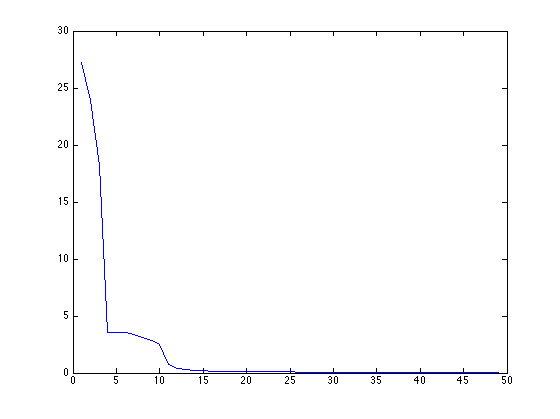
\includegraphics[keepaspectratio=true,scale=0.5]{conj_fx_Bleale.png}}
				\captionof{figure}{Function values of the optimization using conjugate gradient.}   
			\end{minipage}
			
		
		\subsection{Rosenbrock Function}
		This function was difficult to visualize as it contained 4 variables. I plotted the values f(x) at each iteration. We can see that all the functions were minimized to a minimum. BFGS method was the fastest to converge for the experiments that I performed. \\
	\noindent%
	\begin{minipage}{\linewidth}% to keep image and caption on one page
		\makebox[\linewidth]{%        to center the image
			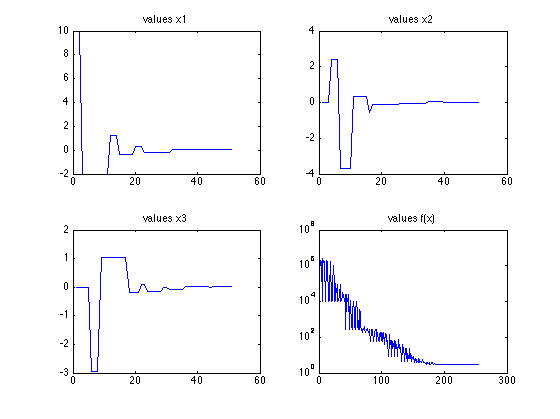
\includegraphics[keepaspectratio=true,scale=0.7]{Nelder_rosen.png}}
		\captionof{figure}{log(f(x)) values for the Nelder-Mead algorithm. I plotted using log so that a mor informative display of the values in relation to the iterations could be seen. We can see the simplex algorithm in action by considering the views of the x1,x2,x3 values. x4 not included.}   
	\end{minipage}
			\noindent%
	\begin{minipage}{\linewidth}% to keep image and caption on one page
		\makebox[\linewidth]{%        to center the image
			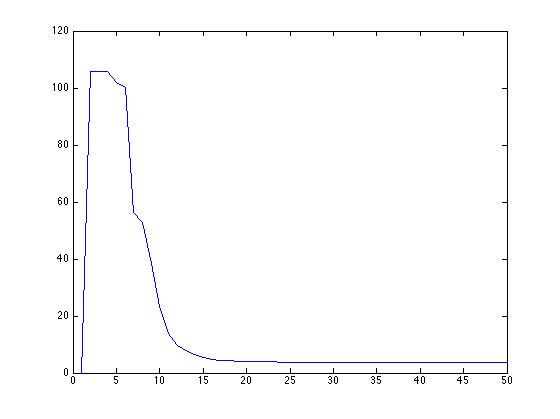
\includegraphics[keepaspectratio=true,scale=0.5]{bfgs_rosen.png}}
		\captionof{figure}{BFGS optimization for the rosen function.}   
	\end{minipage}
			\noindent%
	\begin{minipage}{\linewidth}% to keep image and caption on one page
		\makebox[\linewidth]{%        to center the image
			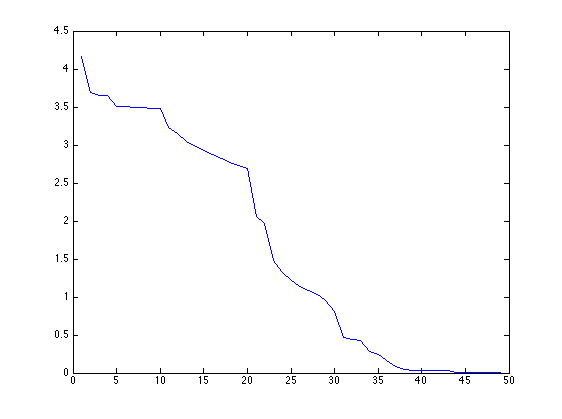
\includegraphics[keepaspectratio=true,scale=0.5]{conjRosenValue.png}}
		\captionof{figure}{non-linear Conjugate gradient method. We see a slower convergence, which is not what we expect.}   
	\end{minipage}
	\section{Lagrange Multipliers} 
	$$ min \sum_{i=1}^n a_i^2x_i \verb|  subject to | \sum_{i=1}^n \frac{1}{x_i-c} -\frac{1}{b}$$
	Following the Lagrangian equation: 
	$$ L(x_i,\lambda = f(x_i) -\lambda(g(x_i) -c) $$
	We get:
	$$L = \sum_{i=1}^n a_i^2x_i -\lambda \sum_{i=1}^n \frac{1}{x_i-c} - \frac{1}{b} $$
	$$ \triangledown L = 0 $$
	$$\triangledown L = \triangledown \sum_{i=1}^n a_i^2x_i -\triangledown \lambda \sum_{i=1}^n \frac{1}{x_i-c} - \frac{1}{b} $$
	$$ = \sum_{i=1}^n a_i^2 \triangledown x_i -\lambda \sum_{i=1}^n \triangledown \frac{1}{x_i-c} - \frac{1}{b} $$
	$$0 = \sum_{i=1}^n a_i^2 - \lambda \sum_{i=1}^n \frac{1}{-(x_i-c)^2}$$
	$$ \lambda = -\sum_{i=1}^n a_i^2 (x_i-c)^2$$
		\end{document} 